\subsection{Die Sprache von Anforderungen}
\label{sec:Kap-6.2.3}

\vspace{2mm} %%% für Druck

In Softwareentwicklungsprojekten werden Anforderungen textuell, grafisch oder als Kombination textueller und grafischer Elemente formuliert. Bei den textuellen Anforderungen reicht die Spannweite von natürlicher Sprache über leicht formalisierte und einheitliche Satzstrukturen bis hin zu festen Anforderungsschablonen.

\vspace{2mm} %%% für Druck

\minisec{Natürliche Sprache}

Die Verwendung natürlicher Sprache hat den Vorteil, dass Kunden ihre Anforderungen aufschreiben können, ohne sich in spezielle Schemata oder Modellierungs\-sprachen einarbeiten zu müssen. Gleichzeitig hat natürliche Sprache das Problem, dass auch mehrdeutige, missverständliche oder schlicht unverständliche Formulierungen sprachlich möglich sind. Typische Probleme entstehen zum Beispiel durch:

\begin{itemize}
	\item die Verwendung mehrerer unterschiedlicher Begriffe für dasselbe Konzept bzw. Anliegen
	\item die Verwendung desselben Begriffs für unterschiedliche Konzepte
	\item die Verkürzung von komplexen Prozessbeschreibungen auf einen Begriff (\zb Buchung, Erfassung, Registrierung, Belegung). Abweichende Vorstellungen \linebreak %%% für Druck
		vom zugrundeliegenden Prozess könnten in Diskussionen unerkannt bleiben, weil alle den identischen Begriff verwenden.
	\item fehlende Angaben, für welche Nutzerrollen eine Anforderung gedacht ist
	\item nicht angegebene Sonderfälle in textuellen Prozess- oder Ablaufbeschreibungen
\end{itemize}

\vspace{2mm} %%% für Druck

Es lohnt sich, zu Beginn eines Softwareentwicklungsprojekts einen gewissen Mehraufwand an Zeit einzuplanen, um mit den Stakeholdern schon für Nutzeranforderungen einfache Regeln für Prosaformulierungen abzusprechen. Bei in Prosa formulierten Systemanforderungen sollte man zusätzlich darauf achten, dass für gewünschte Funktionalitäten benötigte Ein- oder Ausgabedaten und Sonderfälle beschrieben werden.

\vspace{2mm} %%% für Druck

\minisec{Satzschablonen}

%%% Hier gehört die Abbildung "fig:satzschablone_fuer_systemanforderungen" eigentlich hin.

Anforderungen können über sogenannte Satzschablonen auch in unterschiedlich stark strukturierten Formen erfasst werden. Satzschablonen sollen die Eindeutigkeit von Anforderungen erhöhen und dadurch Missverständnisse verringern. Abbildung~\ref{fig:satzschablone_fuer_systemanforderungen} zeigt Beispiele für Satzschablonen. Satzschablonen werden heute überwiegend für die Formulierung von \textbf{System}\-an\-for\-de\-run\-gen eingesetzt, an denen das Softwareentwicklungsteam und die Kunden gemeinsam arbeiten.  

Wenn Sie sich detaillierter mit Satzschablonen beschäftigen möchten, finden Sie bei \cite[59 \psqq]{poh15} und vor allem bei \cite[219 \psqq]{rup14} ausführliche Informationen zum Einsatz von Satzschablonen für funktionale und nichtfunktionale Anforderungen.

\pagebreak %%% für Druck

\begin{figure} [h!]
	\centering
	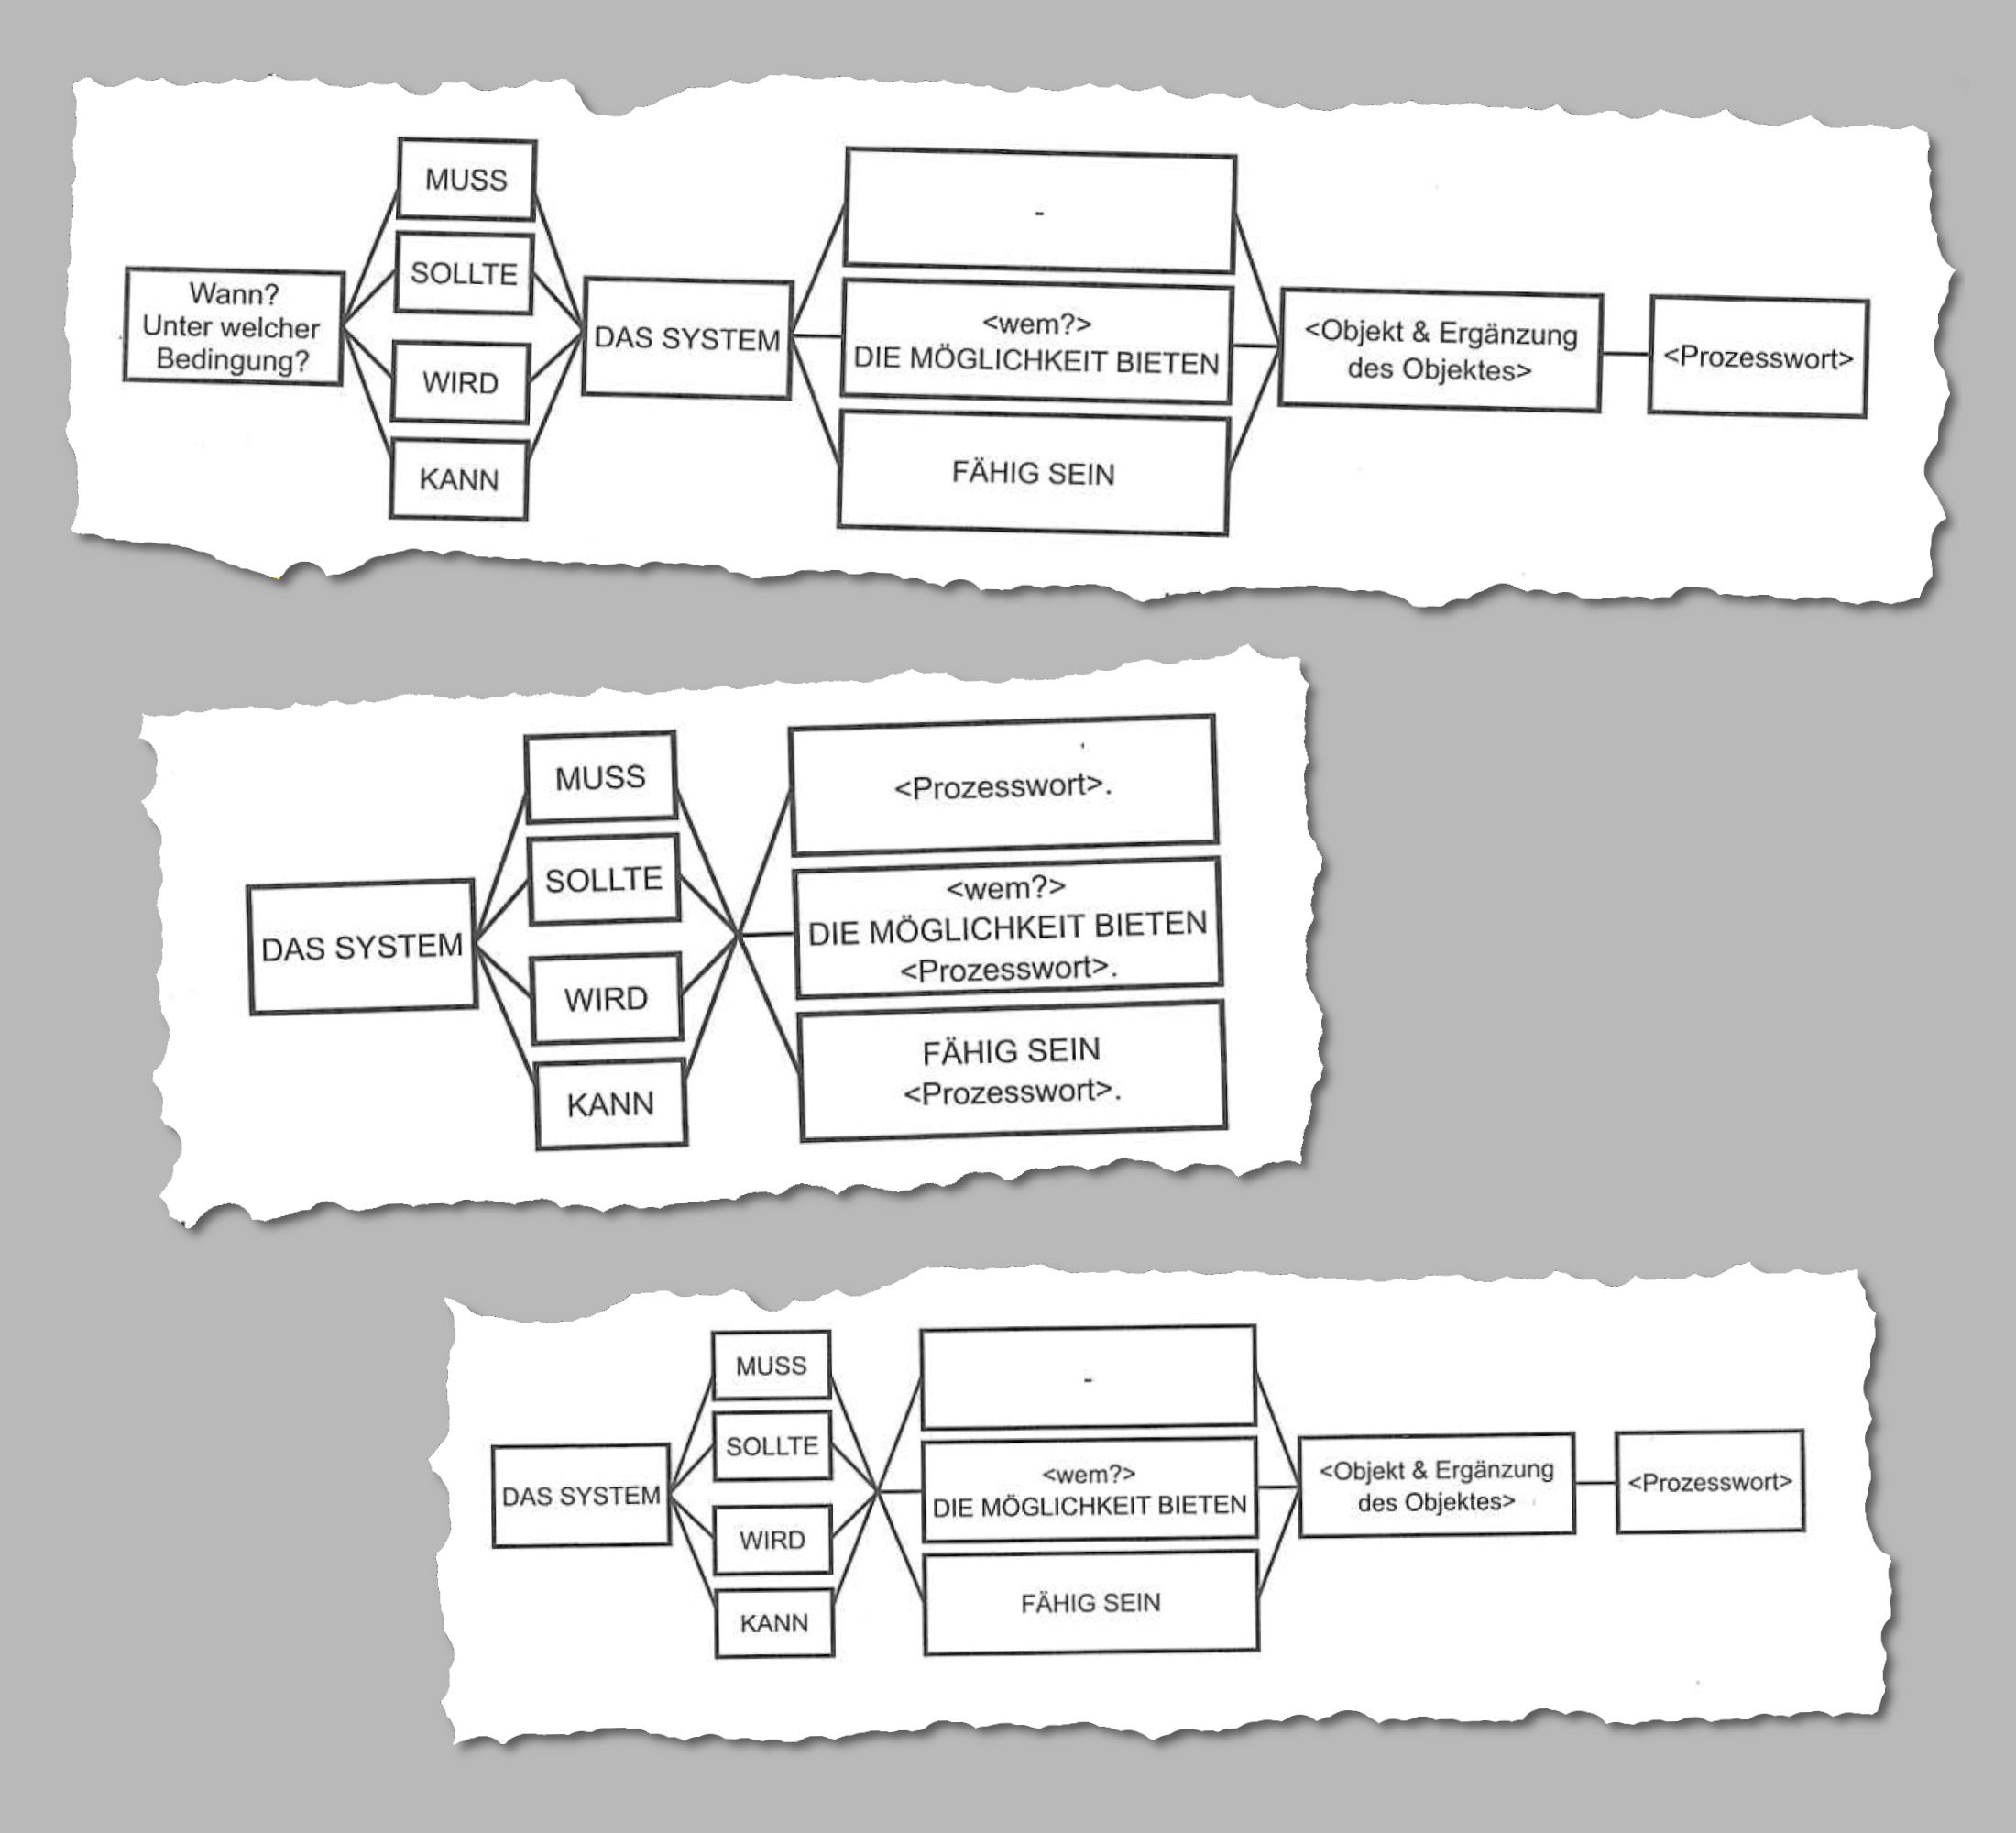
\includegraphics[width=\textwidth]{Bilder/Kapitel-6/Satzschablonen_Medley_V2.png}
	\caption[Satzschablonen]{Satzschablonen \cite[59 \psqq]{poh15}}
	\label{fig:satzschablone_fuer_systemanforderungen}
\end{figure}

\minisec{User Stories}

Insbesondere im agilen Umfeld wird für Nutzeranforderungen -- vor allem wenn sie extern sichtbares Verhalten des Systems betreffen -- eine leicht standardisierte Form gewählt, die beinhaltet, aus dem Blickwinkel welcher Personengruppe die Anforderung gestellt wird und auch explizit angibt, \textbf{warum} die Anforderung gestellt wird:

\sttpAnforderungText{"`Als [Rollenbezeichnung] möchte ich [Aktion], um [Zweck/Ziel/Bedürfnis]"'.}

Zum Beispiel: 

\sttpAnforderungText{"`Als oberster Tierpfleger im Zoo möchte ich die Urlaubs- und Abwesenheitszeiten der Tierpfleger einsehen können, um die wöchentlichen Dienstpläne der Tierpfleger zu erstellen"'.}

Eine solche Anforderungsformulierung nennt man eine \textit{User Story}. User Stories umfassen in der Regel einen oder zwei Sätze und werden in natürlicher Sprache formuliert, häufig in der dargestellten leicht strukturierten Form. Anders als bei den oben erwähnten Satzschablonen ist bei dieser agilen Form einer "`Schablone"' der Aufbau einer Anforderung nur sehr schwach vorstrukturiert. Insbesondere die Aktion, die die Rolle ausführen können möchte, kann in sehr unterschiedlichem Detaillierungsgrad in Form individueller Prosa beschrieben werden. Die Formulierung als User Story erfordert für die Anforderungssteller kaum Einarbeitungsaufwand. Zudem ist sie sehr auf die Arbeitsprozesse und Bedürfnisse des konkreten Anforderungsstellers fokussiert. Dieser explizite Bezug zur Rolle hat den Vorteil, dass unmittelbar deutlich ist, für welche Gruppe eine Funktionalität gewünscht wird. Ein gewisser Motivations\-aspekt für die Anforderungssteller ("`Ich beschreibe die Wünsche \textbf{meiner} Rolle"') ist zusätzlich gegeben.

\vspace{2.5mm} %%% für Druck

So bequem und motivationsfördernd eine solche, nur leicht vorstrukturierte, Erfassung von Anforderungen für die Anforderungssteller ist, desto komplizierter kann sie für den Requirements Engineer, den Product Owner, den Projektleiter oder die sonstige Rolle werden, die die Strukturierung und Priorisierung der Anforderungen im konkreten Softwareentwicklungsprojekt vornimmt: Durch die Fokussierung einer Anforderung auf die Bedürfnisse einer einzelnen Rolle wird der gesamte Prozess der Erfassung von Anforderungen auf einer kleinschrittigen Mikroebene organisiert. Gerade in Projekten mit vielen unterschiedlichen (Nutzer)Rollen kann eine anschließend gewünschte Zuordnung der erfassten Anforderungen zu größeren inhaltlichen Gruppen sehr aufwändig werden. Die unterschiedlichen Anforderungen müssen verglichen und gemeinsame Wünsche, aber auch Inkonsistenzen erkannt werden. Zum Beispiel wird im Zookontext die Rolle oberster Tierpfleger nicht die einzige sein, die Informationen zu den Abwesenheitszeiten der Tierpfleger für ihre Arbeit benötigt. Jede der anderen Rollen (\zb Tierarzt, Tierfütterungsorganisator, Personalverwaltung) wird eine ähnliche Anforderung zu diesem Kontext stellen, aber möglicherweise mit anderer Schwerpunktsetzung und sicher anders formuliert.

\vspace{2.5mm} %%% für Druck

In einem stark agil orientierten Projekt, bei dem die ständige iterative Anpassung sowohl der Anforderungen als auch ihrer Umsetzung in Programmcode zum Tages\-geschäft gehört, würde man zu Beginn des Projekts eine Zuordnung der Anforderungen zu größeren Gruppen gar nicht zwingend vornehmen wollen bzw. können, da die Sammlung weiterer Anforderungen parallel zur Umsetzung schon bestehender Anforderungen weiter läuft. Ein rollenzentriertes kleinschrittiges Vorgehen ist in solchen Projekten daher nicht von Nachteil -- und für solche Projekte sind User \mbox{Stories} auch eingeführt worden. Für Projekte, in denen der Großteil der Anforderungen schon zu Projektbeginn festgelegt werden soll, wird die rollenzentrierte kleinschrittige Erfassung der Anforderungen dagegen maximal der erste Schritt auf dem Weg zur Anforderungsspezifikation sein. %TODO:hier Verweis auf Storymap, wenn nicht in 5.3

\vspace{2.5mm} %%% für Druck

Unbestreitbar sinnvoll -- unabhängig vom gewählten Vorgehensmodell -- ist die in einer User Story vom Anforderungssteller verlangte Angabe des Zwecks seiner Anforderung. Auf diese Weise kann bei der Priorisierung von Anforderungen besser eingeschätzt werden, welche Folgen die Nichtberücksichtigung einer konkreten Anforderung hätte.

\minisec{Grafische Modelle}

Irgendwann im Laufe eines Softwareentwicklungsprozesses kommt der Zeitpunkt, zu dem man von der Ebene natürlichsprachlicher Beschreibungen auf die Ebene von \mbox{Modellen} wechselt. Das kann erst spät erfolgen, wie in vielen agilen Projekten, in denen die Bedürfnisse aus natürlichsprachlichen Anforderungen direkt in Programmcode für Funktionen umgesetzt werden, die diese Bedürfnisse erfüllen. In anderen Projekten werden natürlichsprachliche Anforderungen im Zuge von Entwurfstätigkeiten in (Entwurfs)Modelle übersetzt und dabei verfeinert und erst letztere Modelle dann in Programmcode umgesetzt. Grafische Modelle schon für die Anforderungsermittlung einzusetzen, kann man insofern auch als vorbereitende Arbeiten für Aufgaben ansehen, die man später sowieso erledigen müsste. Die während des Require\-ments Engineering entstandenen Modelle werden dann zu verfeinerten Modellen für Entwurfsbelange weiterentwickelt.

\vspace{1mm} %%% für Druck

Und so werden auch grafische Modelle im Requirements Engineering eingesetzt, um Anforderungen zu erfassen, zum Beispiel in folgenden Kontexten:

\begin{itemize}
	\item Domänenbasierte Anforderungen werden häufig in Form von Klassendiagrammen erfasst. 
	\item Das extern sichtbare Verhalten des Softwaresystems für seine unterschiedlichen Nutzergruppen kann über UML-Anwendungsfalldiagramme erfasst werden.
	\item Geschäftsprozesse, die das zukünftige Softwareprodukt durchführen oder unterstützen soll, werden ebenfalls oft grafisch dargestellt. Aus dem UML-
	\linebreak %%% für Druck
	Universum bieten sich hierfür Aktivitätsdiagramme an. Außerhalb der UML existieren zudem einige spezifische Notationen für die Darstellung von 
	\linebreak %%% für Druck
	Geschäfts\-prozessen.
	\item Anforderungen an die Schnittstellen zu anderen Systemen können über das in Abschnitt~\ref{sec:Kap-6.1.3.1} erwähnte Kontextdiagramm erfasst werden, indem dieses um die Informations- und Datenflüsse zwischen den Systemen ergänzt wird.
\end{itemize}

\vspace{1mm} %%% für Druck

Die gerade aufgezählten Arten von Anforderungen könnten grundsätzlich auch durch textuelle Formen (Prosa oder Satzschablonen) erfasst werden. Der Vorteil von grafischen Modellen gegenüber der natürlichen Sprache ist ihr höherer Grad an Eindeutigkeit, weil sie in der Regel viel weniger Interpretationsspielraum zulassen als natürliche Sprache. Zudem lassen sich Anforderungen, die man textuell sehr ausführlich beschreiben müsste (\zb komplexe Geschäftsprozesse) häufig mit grafischen Modellen einfacher und übersichtlicher darstellen. Ein Nachteil für die Adressaten ist der Einarbeitungsaufwand in die verwendete Modellierungssprache. Ein weiterer Nachteil ist der höhere Aufwand für die Pflege und Anpassung von Modellen: Eine natürlichsprachliche Anforderung kann mit wenig Aufwand umformuliert werden. Bei einer Anforderung, die Teil eines Modells ist, müssen bei jeder Änderung die Einhaltung der syntaktischen und semantischen Regeln der Modellierungssprache und die Auswirkungen auf andere Anforderungen im Modell berücksichtigt werden.

\vspace{1mm} %%% für Druck

Letzterer Aspekt adressiert schon einen grundlegenden Unterschied im Einsatzzweck zwischen der Verwendung textueller (vor allem natürlichsprachlicher) Formulierungen und der Verwendung von grafischen Modellen: Grafische Modelle werden häufig in Situationen eingesetzt, in denen weniger eine einzelne Anforderung im Fokus steht, als vielmehr Gruppen von Anforderungen und ihre Beziehungen zueinander betrachtet werden. Zusammenhänge zwischen einzelnen Anforderungen würden sich zwar auch in natürlichsprachlichen Formulierungen ausdrücken lassen, aber grafische Modelle bieten hier eine deutlich bessere Übersichtlichkeit. Auf diese Weise können widerstreitende Anforderungen einfacher erkannt werden oder zum Beispiel auch (Geschäfts)Bereiche identifiziert werden, aus denen bisher nur wenige Anforderungen vorliegen. In der Praxis werden grafische Modellform und textuelle Formulierungen häufig kombiniert, um die grafischen Modelle mit zusätzlichen Informationen anzureichern. Letztere werden dann aber meist in einer strukturierten textuellen Form und nicht in Prosa erfasst.

\vspace{2mm} %%% für Druck

\minisec{Das Anforderungsdiagramm von SysML}

\vspace{1mm} %%% für Druck

Wir haben oben kurz skizziert, welche UML-Diagramme man für die Erfassung verschiedener Arten von Anforderungen einsetzen kann. Ein spezifisches Anforderungsdiagramm besitzt die UML nicht. Ein solches findet sich allerdings in der Systems Modeling Language (SysML, \url{https://www.omgsysml.org/}), die im Jahr 2007 ebenfalls von der OMG veröffentlicht wurde. Während die UML schwerpunktmäßig auf die reine Softwareentwicklung ausgerichtet ist, nimmt die SysML mit der kompletten Systementwicklung (Software, Hardware, Elektronik und Mechanik) technischer Systeme ein deutlich größeres Anwendungsgebiet in den Blick. Die SysML wird heute häufig in Kombination mit Vorgehensweisen der modellgetriebenen System\-entwicklung eingesetzt, für die Systemzusammenhänge aufgrund automatisierter Verarbeitungsschritte auch formal spezifiziert werden müssen. 

\vspace{1mm} %%% für Druck

Für die SysML wurden bestehende UML-Diagramme angepasst und manche -- wie das Anforderungsdiagramm -- neu eingeführt. Die Anforderungen selber werden in einem, an das UML-Klassenelement angelehnten, Element aufgeschrieben und sind so in einer grafisch-textuellen Mischform dargestellt. Ein Vorteil des Anwendungsfalldiagramms ist, dass im selben Diagramm sowohl die Anforderungen und ihre Beziehungen untereinander, als auch Beziehungen zu Elementen anderer UML-Diagrammarten, wie zum Beispiel Anwendungsfälle, modelliert werden können. Das Anforderungsdiagramm kann somit auch Inhalte mehrerer Diagramme und ihre \mbox{Zusammenhänge} in einer Übersicht vereinen. Allerdings wird es dadurch auch deutlich komplexer, schwieriger zu erstellen und weniger intuitiv zu verstehen. In reinen Softwareentwicklungsprojekten wird das SysML-Anforderungsdiagramm daher auch eher selten eingesetzt -- insbesondere kaum für Diskussionen mit den Kunden. Hilfreich kann es für interne Diskussionen des Entwicklungsteams sein, um Abhängigkeiten zwischen verschiedenen nichtfunktionalen Anforderungen zu visualisieren oder Auswirkungen nichtfunktionaler Anforderungen auf funktionale Anforderungen darzustellen. 

\vspace{1mm} %%% für Druck

Eine kurze Übersicht zum SysML-Anforderungsdiagramm liefert \cite[51-53]{alt12}. Einen ausführlichen Blick auf das Diagramm und seine konkrete Verwendung im Rahmen eines vorgestellten Systementwicklungsmodells wirft \cite[234 \psqq]{wei14}.